\documentclass[12pt]{article}
\usepackage{amsmath}
\usepackage{tikz}
\begin{document}
\title{Computer Science 181, Homework 6}
\date{May 14th, 2018}
\author{Michael Wu\\UID: 404751542}
\maketitle

\section*{Problem 1}

\paragraph{a)}

\begin{align*}
G&=(V,\Sigma,R,S)\\
V&=\{A,B\}\\
R&=\{A\rightarrow \text{a}A\text{d} \mid B,\\
&\hphantom{==}B\rightarrow \text{b}B\text{c} \mid \epsilon\}\\
S&=A
\end{align*}
This context free grammar works in two stages. In the first, we start with the symbol \(A\), which can produce matching pairs of a symbols and d symbols.
It recurses into itself, so that an arbitrary number \(n\geq0\) of matching a's and d's can be generated. There is no production rule for \(\epsilon\) in this first
stage, as that would make the grammar ambiguous. In order to terminate, the grammar has to move into the second stage by producing a symbol \(B\). The second stage
works like the first in that it can generate an arbitrary number \(m\geq0\) of matching b's and c's, but it has a rule for \(\epsilon\) so that it can terminate.
Thus this grammar is unambiguous because there can be only one way to generate a string in the language defined by \(a^nb^mc^md^n\), which is by applying
\(A\rightarrow \text{a}A\text{d}\) for \(n\) times, then \(A\rightarrow B\), then \(B\rightarrow \text{b}B\text{c}\) for \(m\) times, then \(B\rightarrow \epsilon\).

\paragraph{b)}

Define the stack symbols to be \(\Gamma=\{s,n,m\}\). Then the PDA can be drawn as shown below.
\begin{center}
        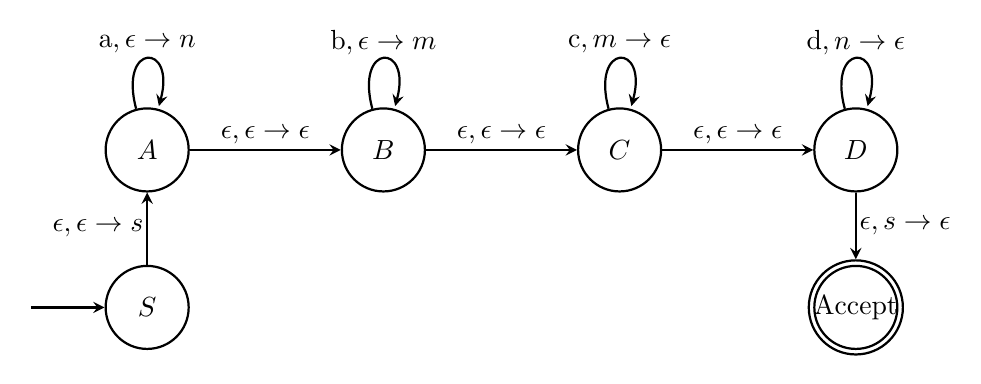
\begin{tikzpicture}
                \begin{scope}[auto, every node/.style={thick, draw,circle,minimum size=3em,inner sep=1}]
                        \node (S) at (0,0) {\(S\)};
                        \node (A) at (0,2) {\(A\)};
                        \node (B) at (3,2) {\(B\)};
                        \node (C) at (6,2) {\(C\)};
                        \node (D) at (9,2) {\(D\)};
                        \node (Accept) at (9,0) {Accept};
                        \draw[black, thick] (9,0) circle [radius=1.5em];
                \end{scope}
                \node [draw=none, inner sep=0pt] (I) at (-1.5,0) {};
                \begin{scope}[auto, every node/.style={minimum size=1em,inner sep=1}, every path/.style={thick, ->, >=stealth}]
                        \path (I) edge (S);
                        \path (S) edge node {\(\epsilon, \epsilon\rightarrow s\)} (A);
                        \path (A) edge [loop above] node {\(\text{a}, \epsilon\rightarrow n\)} (A);
                        \path (A) edge node {\(\epsilon, \epsilon\rightarrow\epsilon\)} (B);
                        \path (B) edge [loop above] node {\(\text{b}, \epsilon\rightarrow m\)}(B);
                        \path (B) edge node {\(\epsilon, \epsilon\rightarrow\epsilon\)} (C);
                        \path (C) edge [loop above] node {\(\text{c}, m\rightarrow\epsilon\)}(C);
                        \path (C) edge node {\(\epsilon, \epsilon\rightarrow\epsilon\)} (D);
                        \path (D) edge [loop above] node {\(\text{d}, n\rightarrow\epsilon\)}(D);
                        \path (D) edge node {\(\epsilon, s\rightarrow\epsilon\)}(Accept);
                \end{scope}
        \end{tikzpicture}
\end{center}

\end{document}